% Options for packages loaded elsewhere
\PassOptionsToPackage{unicode}{hyperref}
\PassOptionsToPackage{hyphens}{url}
\documentclass[
  preprint,12pt]{elsarticle}
\usepackage{xcolor}
\usepackage[margin=1in]{geometry}
\usepackage{amsmath,amssymb}
\setcounter{secnumdepth}{5}
\usepackage{iftex}
\ifPDFTeX
  \usepackage[T1]{fontenc}
  \usepackage[utf8]{inputenc}
  \usepackage{textcomp} % provide euro and other symbols
\else % if luatex or xetex
  \usepackage{unicode-math} % this also loads fontspec
  \defaultfontfeatures{Scale=MatchLowercase}
  \defaultfontfeatures[\rmfamily]{Ligatures=TeX,Scale=1}
\fi
\usepackage{lmodern}
\ifPDFTeX\else
  % xetex/luatex font selection
  \setmainfont[]{Times New Roman}
  \setmathfont[]{STIX Two Math}
\fi
% Use upquote if available, for straight quotes in verbatim environments
\IfFileExists{upquote.sty}{\usepackage{upquote}}{}
\IfFileExists{microtype.sty}{% use microtype if available
  \usepackage[]{microtype}
  \UseMicrotypeSet[protrusion]{basicmath} % disable protrusion for tt fonts
}{}
\makeatletter
\@ifundefined{KOMAClassName}{% if non-KOMA class
  \IfFileExists{parskip.sty}{%
    \usepackage{parskip}
  }{% else
    \setlength{\parindent}{0pt}
    \setlength{\parskip}{6pt plus 2pt minus 1pt}}
}{% if KOMA class
  \KOMAoptions{parskip=half}}
\makeatother
\usepackage{color}
\usepackage{fancyvrb}
\newcommand{\VerbBar}{|}
\newcommand{\VERB}{\Verb[commandchars=\\\{\}]}
\DefineVerbatimEnvironment{Highlighting}{Verbatim}{commandchars=\\\{\}}
% Add ',fontsize=\small' for more characters per line
\newenvironment{Shaded}{}{}
\newcommand{\AlertTok}[1]{\textcolor[rgb]{1.00,0.00,0.00}{\textbf{#1}}}
\newcommand{\AnnotationTok}[1]{\textcolor[rgb]{0.38,0.63,0.69}{\textbf{\textit{#1}}}}
\newcommand{\AttributeTok}[1]{\textcolor[rgb]{0.49,0.56,0.16}{#1}}
\newcommand{\BaseNTok}[1]{\textcolor[rgb]{0.25,0.63,0.44}{#1}}
\newcommand{\BuiltInTok}[1]{\textcolor[rgb]{0.00,0.50,0.00}{#1}}
\newcommand{\CharTok}[1]{\textcolor[rgb]{0.25,0.44,0.63}{#1}}
\newcommand{\CommentTok}[1]{\textcolor[rgb]{0.38,0.63,0.69}{\textit{#1}}}
\newcommand{\CommentVarTok}[1]{\textcolor[rgb]{0.38,0.63,0.69}{\textbf{\textit{#1}}}}
\newcommand{\ConstantTok}[1]{\textcolor[rgb]{0.53,0.00,0.00}{#1}}
\newcommand{\ControlFlowTok}[1]{\textcolor[rgb]{0.00,0.44,0.13}{\textbf{#1}}}
\newcommand{\DataTypeTok}[1]{\textcolor[rgb]{0.56,0.13,0.00}{#1}}
\newcommand{\DecValTok}[1]{\textcolor[rgb]{0.25,0.63,0.44}{#1}}
\newcommand{\DocumentationTok}[1]{\textcolor[rgb]{0.73,0.13,0.13}{\textit{#1}}}
\newcommand{\ErrorTok}[1]{\textcolor[rgb]{1.00,0.00,0.00}{\textbf{#1}}}
\newcommand{\ExtensionTok}[1]{#1}
\newcommand{\FloatTok}[1]{\textcolor[rgb]{0.25,0.63,0.44}{#1}}
\newcommand{\FunctionTok}[1]{\textcolor[rgb]{0.02,0.16,0.49}{#1}}
\newcommand{\ImportTok}[1]{\textcolor[rgb]{0.00,0.50,0.00}{\textbf{#1}}}
\newcommand{\InformationTok}[1]{\textcolor[rgb]{0.38,0.63,0.69}{\textbf{\textit{#1}}}}
\newcommand{\KeywordTok}[1]{\textcolor[rgb]{0.00,0.44,0.13}{\textbf{#1}}}
\newcommand{\NormalTok}[1]{#1}
\newcommand{\OperatorTok}[1]{\textcolor[rgb]{0.40,0.40,0.40}{#1}}
\newcommand{\OtherTok}[1]{\textcolor[rgb]{0.00,0.44,0.13}{#1}}
\newcommand{\PreprocessorTok}[1]{\textcolor[rgb]{0.74,0.48,0.00}{#1}}
\newcommand{\RegionMarkerTok}[1]{#1}
\newcommand{\SpecialCharTok}[1]{\textcolor[rgb]{0.25,0.44,0.63}{#1}}
\newcommand{\SpecialStringTok}[1]{\textcolor[rgb]{0.73,0.40,0.53}{#1}}
\newcommand{\StringTok}[1]{\textcolor[rgb]{0.25,0.44,0.63}{#1}}
\newcommand{\VariableTok}[1]{\textcolor[rgb]{0.10,0.09,0.49}{#1}}
\newcommand{\VerbatimStringTok}[1]{\textcolor[rgb]{0.25,0.44,0.63}{#1}}
\newcommand{\WarningTok}[1]{\textcolor[rgb]{0.38,0.63,0.69}{\textbf{\textit{#1}}}}
\usepackage{longtable,booktabs,array}
\newcounter{none} % for unnumbered tables
\usepackage{calc} % for calculating minipage widths
% Correct order of tables after \paragraph or \subparagraph
\usepackage{etoolbox}
\makeatletter
\patchcmd\longtable{\par}{\if@noskipsec\mbox{}\fi\par}{}{}
\makeatother
% Allow footnotes in longtable head/foot
\IfFileExists{footnotehyper.sty}{\usepackage{footnotehyper}}{\usepackage{footnote}}
\makesavenoteenv{longtable}
\usepackage{graphicx}
\makeatletter
\newsavebox\pandoc@box
\newcommand*\pandocbounded[1]{% scales image to fit in text height/width
  \sbox\pandoc@box{#1}%
  \Gscale@div\@tempa{\textheight}{\dimexpr\ht\pandoc@box+\dp\pandoc@box\relax}%
  \Gscale@div\@tempb{\linewidth}{\wd\pandoc@box}%
  \ifdim\@tempb\p@<\@tempa\p@\let\@tempa\@tempb\fi% select the smaller of both
  \ifdim\@tempa\p@<\p@\scalebox{\@tempa}{\usebox\pandoc@box}%
  \else\usebox{\pandoc@box}%
  \fi%
}
% Set default figure placement to htbp
\def\fps@figure{htbp}
\makeatother
\setlength{\emergencystretch}{3em} % prevent overfull lines
\providecommand{\tightlist}{%
  \setlength{\itemsep}{0pt}\setlength{\parskip}{0pt}}
\usepackage{graphicx}
\usepackage{bookmark}
\IfFileExists{xurl.sty}{\usepackage{xurl}}{} % add URL line breaks if available
\urlstyle{same}
\hypersetup{
  pdftitle={VoltGuard-ECM: A DMS Integration Architecture for AC-Audited Voltage-Risk Screening in High-DER Distribution Networks},
  pdfauthor={Siqiang Zhao (corresponding author), Fengxiang Zhang},
  hidelinks,
  pdfcreator={LaTeX via pandoc}}

\title{VoltGuard-ECM: A DMS Integration Architecture for AC-Audited
Voltage-Risk Screening in High-DER Distribution Networks}
\author{Siqiang Zhao (corresponding author), Fengxiang Zhang}
\date{Generated 2026-07-03 02:31 UTC}

\begin{document}
\maketitle

\section*{Title Page}\label{title-page}
\addcontentsline{toc}{section}{Title Page}

\textbf{Journal:} Energy Conversion and Management

\textbf{Article title:} VoltGuard-ECM: A DMS Integration Architecture
for AC-Audited Voltage-Risk Screening in High-DER Distribution Networks

\textbf{Authors and affiliations:}

Siqiang Zhao\(^{a,*}\); Fengxiang Zhang\(^{b}\)

\(^{a}\) Sichuan University-Pittsburgh Institute, Chengdu, China

\(^{b}\) Southwest Jiaotong University, Chengdu, China

\(^{*}\) Corresponding author. Email: 2023141520257@stu.scu.edu.cn

\section*{Abstract}\label{abstract}
\addcontentsline{toc}{section}{Abstract}

High-DER distribution operation requires distribution management systems
(DMS) to triage many forecasted feeder states before committing
expensive AC power flow, OPF, or MPC studies. This paper addresses a
system-integration question rather than a new learning-method question:
how should a calibrated voltage-risk screen be embedded into a DMS so
that release, watch, and corrective-audit decisions remain auditable?
VoltGuard-ECM specifies an integration architecture, input data
contract, queue semantics, exception rules, algorithmic decision logic,
rolling drift audit, and AC-audit handoff for a screening layer placed
between forecast ingestion and trusted corrective tools. The paper
deliberately does not reuse the core prediction, calibration, and
release metrics of the companion method study. Its contribution is the
engineering envelope that makes any calibrated screen deployable: input
validity checks, queue labels, operator override logic, rolling drift
audit, and mandatory fallback to AC analysis under stale telemetry,
unseen topology, or out-of-envelope DER forecasts. A seven-day Python
prototype processes 1008 simulated operating cycles and demonstrates
release/watch/corrective-audit queue assignment, fallback routing,
operator override logging, and drift-alarm records. VoltGuard-ECM is
therefore a DMS-facing governance layer for voltage-risk screening, not
a claim that a screen replaces AC feasibility analysis or optimal
control.

\section*{Keywords}\label{keywords}
\addcontentsline{toc}{section}{Keywords}

Distribution operation; Voltage-risk screening; DMS integration; Queue
semantics; DER operation; AC audit; Fallback rules

\section{Engineering Motivation}\label{engineering-motivation}

Distribution control rooms increasingly receive batches of PV, EV,
storage, and flexible-load forecasts. A conservative workflow sends
every forecasted state to AC power flow or corrective optimization. That
workflow is robust but can be inefficient when many scenarios are
clearly far from voltage limits. A screening layer is attractive only if
it can be integrated without weakening operator accountability.

This paper asks a different question from a method paper. It does not
ask which residual learner or conformal grouping gives the best
interval. It asks: what DMS contract is needed before a voltage-risk
screen can safely influence release, watch, and audit queues?

The answer is an architecture. VoltGuard-ECM treats the screen as a
governed front end. It receives forecast and topology objects, returns
auditable queue records, and triggers fallback rules whenever the inputs
or residual behavior fall outside the calibrated envelope.

This is the DMS companion paper to the VoltGuard screening-method study
and the LinDistFlow-global-quantile baseline note. The method paper
defines how calibrated intervals are estimated; the baseline note
defines a transparent reference screen; this paper defines the
operational contract required before any such screen may influence DMS
queues.

\section{Engineering Context}\label{engineering-context}

Distribution operation already relies on AC power flow, state
estimation, operator rules, voltage margins, OPF, and corrective
control. These tools remain the authority for feasibility. A screening
layer can reduce workload only if it is subordinate to those tools and
if every release decision remains traceable.

The integration challenge is therefore not only computational. It is
also a data-governance problem. The screen must know which feeder model
was used, which topology state is active, which forecasts are fresh,
which calibration protocol applies, and when the result should be
ignored. Without this contract, a strong offline predictor can become
unsafe in deployment because the DMS cannot tell whether the current
state is comparable to calibration.

\subsection{Acronym Table}\label{acronym-table}

{\def\LTcaptype{none} % do not increment counter
\begin{longtable}[]{@{}ll@{}}
\toprule\noalign{}
Acronym & Meaning \\
\midrule\noalign{}
\endhead
\bottomrule\noalign{}
\endlastfoot
AC & alternating-current power flow model \\
AMI & advanced metering infrastructure \\
CIM & common information model \\
DER & distributed energy resource \\
DMS & distribution management system \\
EV & electric vehicle \\
IEC & International Electrotechnical Commission \\
MPC & model predictive control \\
OPF & optimal power flow \\
PV & photovoltaic generation \\
SCADA & supervisory control and data acquisition \\
\end{longtable}
}

\subsection{DMS Integration Standards and
Protocols}\label{dms-integration-standards-and-protocols}

The architecture should be mapped to existing utility data standards
rather than implemented as an isolated ML service. IEC 61970/61968 CIM
objects {[}27,28{]} can carry network models, equipment identifiers,
measurements, switch states, and asset metadata. IEEE 2030.5 {[}29{]}
can represent DER communication and control interfaces in customer-side
or aggregator-connected settings. OpenFMB-style {[}30{]} field-message
patterns can support distributed message exchange when feeder devices,
edge applications, and control-room services share a common operational
model. VoltGuard-ECM does not prescribe one vendor stack; it specifies
the minimum screening fields that must survive translation into those
standards: model version, topology id, forecast timestamp, calibration
protocol, queue label, reason code, operator override, and downstream AC
outcome.

\subsection{Generalization to Other Screening
Methods}\label{generalization-to-other-screening-methods}

The architecture is designed for VoltGuard but is not
VoltGuard-specific. A LinDistFlow-global-quantile screen, a
sensitivity-factor screen, a quantile regression model, or a future
OPF-assisted classifier can plug into the DMS contract if it exposes
four outputs: a scenario risk score, bus-level risk flags or voltage
intervals, a calibration/envelope identifier, and a reason code when the
screen declines to release a scenario. The DMS should treat the screen
as an interchangeable module and should validate each module with the
same queue, fallback, audit, and drift-monitoring tests.

\subsection{Related Integration Work and
Positioning}\label{related-integration-work-and-positioning}

Prior work on DMS and energy-management integration can be grouped into
four technical lines. First, model-exchange standards such as CIM, IEEE
2030.5, and OpenFMB define how grid assets, measurements, DER messages,
and field devices should be represented, but they do not specify how an
ML-based voltage screen should decide release, watch, and audit queues.
Second, conventional DMS analytics rely on state estimation, AC power
flow, OPF, and operator voltage margins. These tools remain
authoritative, yet they can be computationally expensive when every
forecasted DER scenario is audited with full AC analysis. Third,
edge-computing and federated-learning studies for distribution systems
address where analytics may run and how data can be shared, but they
often leave queue semantics, reason codes, and operator overrides
underspecified. Fourth, ML voltage-prediction papers report offline
accuracy, whereas deployment requires input-validity checks,
model-version binding, and post-decision audit records.

VoltGuard-ECM is positioned at this integration boundary. It does not
replace the standards or the AC tools; it defines the missing
operational envelope that allows a calibrated screen to become a
traceable DMS object.

{\def\LTcaptype{none} % do not increment counter
\begin{longtable}[]{@{}
  >{\raggedright\arraybackslash}p{(\linewidth - 6\tabcolsep) * \real{0.2500}}
  >{\raggedright\arraybackslash}p{(\linewidth - 6\tabcolsep) * \real{0.2500}}
  >{\raggedright\arraybackslash}p{(\linewidth - 6\tabcolsep) * \real{0.2500}}
  >{\raggedright\arraybackslash}p{(\linewidth - 6\tabcolsep) * \real{0.2500}}@{}}
\toprule\noalign{}
\begin{minipage}[b]{\linewidth}\raggedright
Integration line
\end{minipage} & \begin{minipage}[b]{\linewidth}\raggedright
Main contribution
\end{minipage} & \begin{minipage}[b]{\linewidth}\raggedright
Gap for voltage-risk screening
\end{minipage} & \begin{minipage}[b]{\linewidth}\raggedright
VoltGuard-ECM role
\end{minipage} \\
\midrule\noalign{}
\endhead
\bottomrule\noalign{}
\endlastfoot
CIM / IEEE 2030.5 / OpenFMB standards & interoperable grid and DER data
objects & no queue or fallback policy for screening outputs & maps
screen records to auditable fields \\
AC PF / OPF / MPC in DMS & trusted feasibility and corrective decisions
& expensive for high-volume forecast triage & preserves AC audit as
backend authority \\
Edge and federated grid analytics & deployment location and data-sharing
pattern & weak operator-facing semantics & adds release/watch/audit
reason codes \\
ML voltage prediction papers & offline point or interval estimates &
limited DMS governance and drift logging & wraps calibrated screens in a
DMS contract \\
\end{longtable}
}

\section{System Integration
Architecture}\label{system-integration-architecture}

VoltGuard-ECM contains five DMS-facing interfaces.

First, the forecast interface receives load, PV, EV, storage, and
flexible-load forecasts or pseudo-measurements with timestamps and
provenance. Each forecast record must identify the operating horizon,
data source, freshness, and quality flags.

Second, the network-model interface receives feeder topology, branch
impedances, slack-bus voltage, switch states, voltage limits, and DER
connection metadata. The screening layer must bind every result to a
specific model version and topology identifier.

Third, the screening interface computes voltage-risk intervals or
point-risk flags using the active screening module selected by the
operator. The architecture is method-agnostic: the module can be a
LinDistFlow baseline, residual learner, conformal interval estimator, or
another calibrated screen.

Fourth, the queue interface maps scenario-level outputs to release,
watch, and corrective-audit queues. The release queue is only advisory:
it means that the scenario does not require immediate AC audit under the
current envelope. The watch queue preserves cases close to limits or
affected by mild input uncertainty. The corrective-audit queue sends
cases to AC power flow, OPF, MPC, or operator review.

Fifth, the audit interface records the decision path. Each record stores
the scenario identifier, model version, calibration protocol,
input-validity checks, risk score, queue label, operator override if
present, and downstream AC outcome once available.

The complete workflow is: forecast ingestion; CIM/topology binding;
input validity checks; screening-module execution; fallback-rule
evaluation; queue assignment; operator review or override; AC
power-flow/OPF/MPC handoff for audited cases; downstream outcome
logging; and rolling residual/drift update. The graphical workflow in
Figure 1 gives the high-level flow, while the algorithms below specify
the executable decision logic.

\begin{figure}
\centering
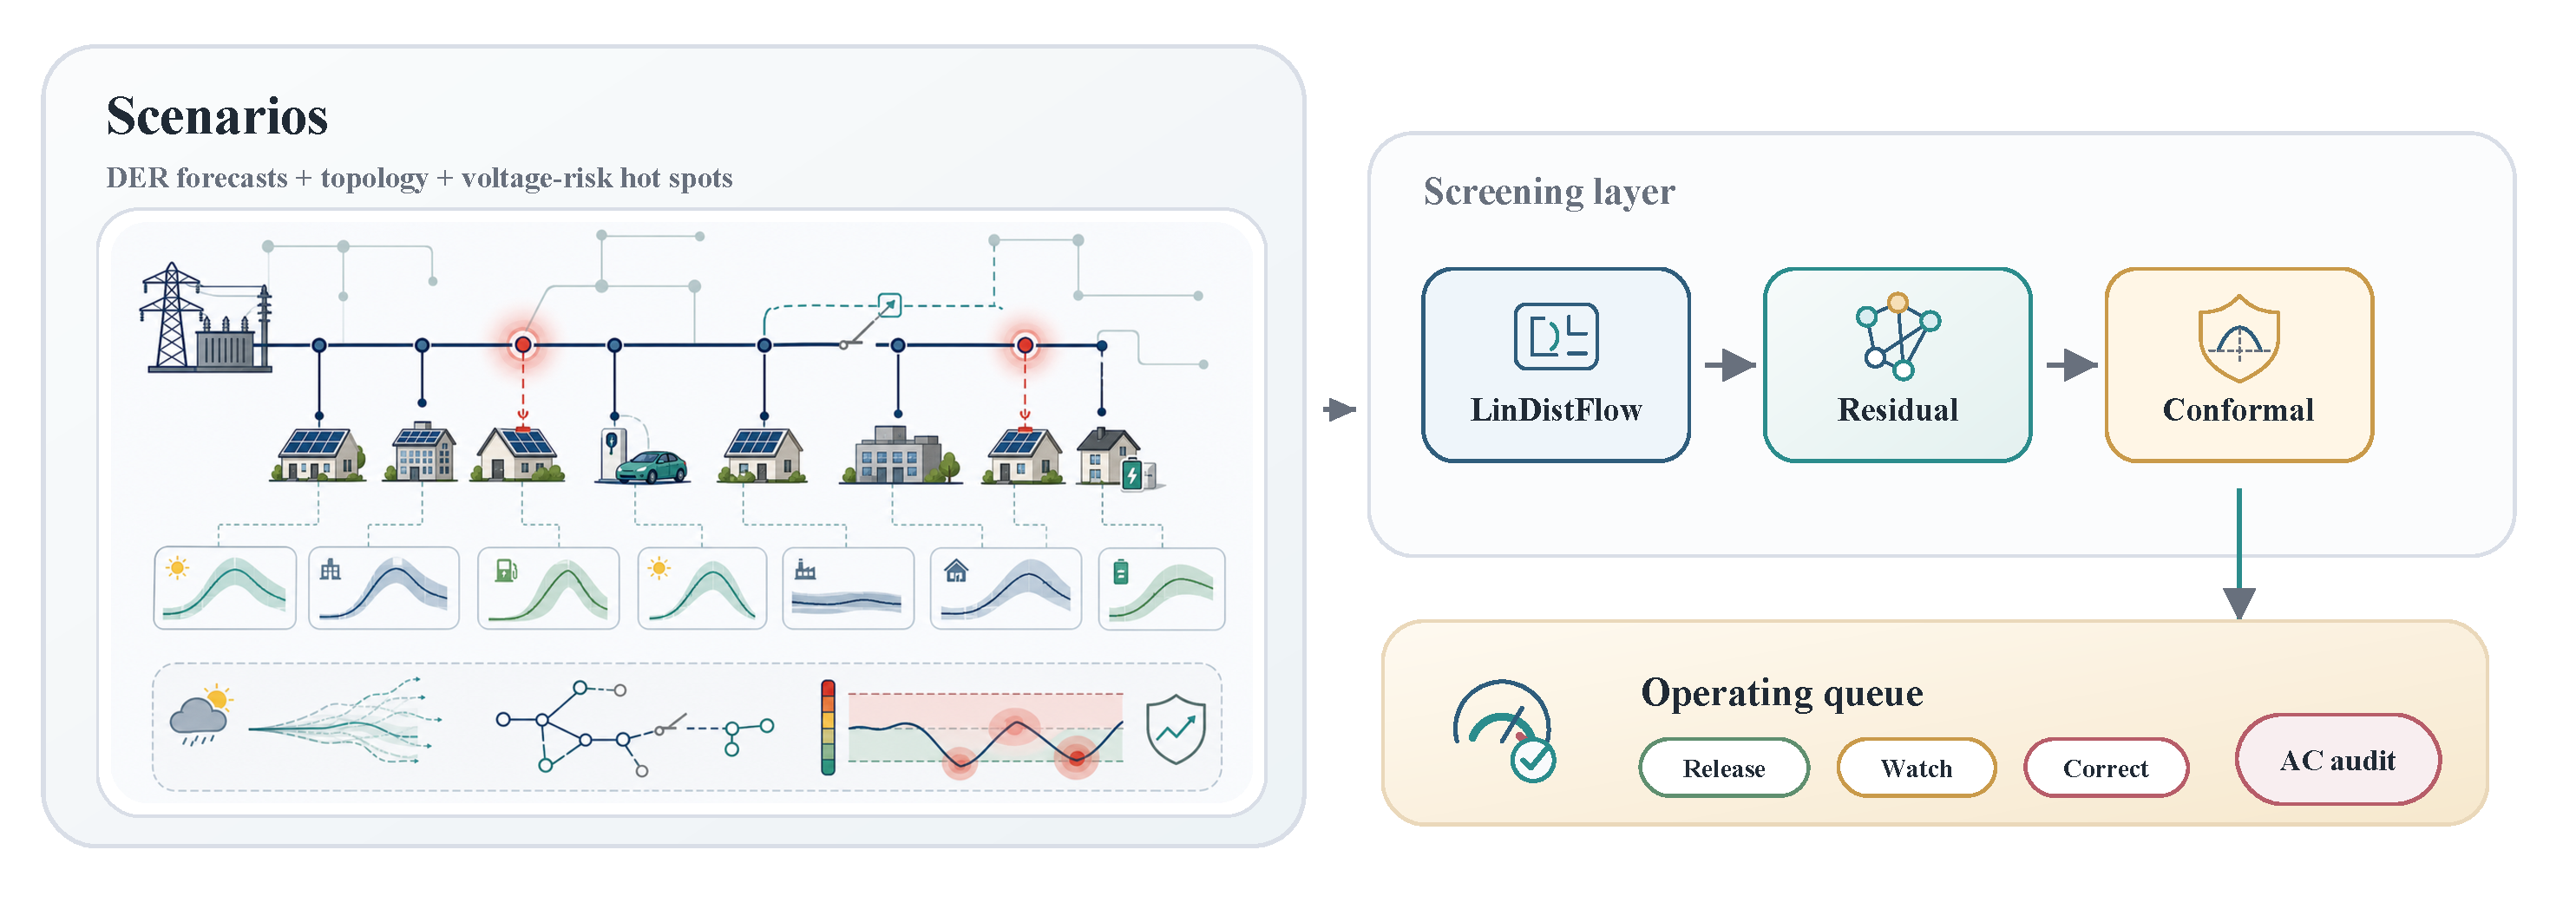
\includegraphics[width=1.1\linewidth,height=\textheight,keepaspectratio,alt={Graphical abstract and VoltGuard screening workflow. The figure summarizes the active-feeder inputs, LinDistFlow physical backbone, topology-aware residual correction, conformal voltage-risk intervals, and downstream AC-audited corrective optimization interface.}]{figures/fig01_graphical_abstract_workflow.pdf}
\caption{Graphical abstract and VoltGuard screening workflow. The figure
summarizes the active-feeder inputs, LinDistFlow physical backbone,
topology-aware residual correction, conformal voltage-risk intervals,
and downstream AC-audited corrective optimization
interface.}\label{fig:fig01_graphical_abstract_workflow}
\end{figure}

\section{Stakeholder Requirements}\label{stakeholder-requirements}

Operators need a screen they can interrogate. Every release, watch, or
audit record should show the active topology, the voltage-limit margin,
the reason code, and whether the result came from a calibrated family or
a fallback rule. The system should minimize nuisance alarms, but
operator trust depends more on clear escalation rules than on a single
offline accuracy number.

Utility IT teams need cybersecurity, access control, logging, and data
lineage. Screening modules should run with least-privilege access,
receive signed model artifacts, write immutable audit records, and avoid
storing unnecessary customer-level data outside approved systems. Model
files, calibration sets, and queue records should have retention
policies consistent with the utility's operational data-governance
program.

Regulators and compliance auditors need accountability. The DMS must be
able to reconstruct why a scenario was released or sent to AC audit,
which model version was active, whether an operator overrode the queue
label, and what the downstream AC result showed. Black-box predictions
are therefore insufficient; the screening layer must produce traceable
decisions.

\section{Queue Semantics}\label{queue-semantics}

\subsection{Release Queue}\label{release-queue}

A released scenario is not certified feasible. It is a scenario that the
screening layer considers low priority for immediate AC audit under the
active calibration envelope. Release records should include the interval
margin to voltage limits, the active topology identifier, and the
input-validity status. Operators may still sample released scenarios for
periodic AC audit to detect silent drift.

\subsection{Watch Queue}\label{watch-queue}

The watch queue is the buffer between release and corrective audit.
Scenarios enter this queue when intervals are near voltage limits,
forecast quality is degraded, or recent residual monitoring suggests
mild distribution shift. The DMS can route watch scenarios to delayed AC
audit, operator review, or additional measurement collection.

\subsection{Corrective-Audit Queue}\label{corrective-audit-queue}

The corrective-audit queue is mandatory when intervals intersect voltage
limits, input checks fail, topology is unseen, or telemetry is stale.
The screen does not prescribe the final action. It supplies the
scenario, suspected buses, direction of voltage risk, and ranking
metadata to the downstream AC tool.

\section{Fallback and Drift
Governance}\label{fallback-and-drift-governance}

VoltGuard-ECM uses conservative fallback rules because calibrated
screens are protocol-dependent. The following conditions bypass release
and trigger AC audit or operator review:

\begin{itemize}
\tightlist
\item
  feeder topology is missing, stale, or absent from the calibration
  envelope;
\item
  forecast timestamps exceed the DMS freshness limit;
\item
  PV, EV, storage, or load features lie outside calibrated ranges;
\item
  online residual monitors exceed a rolling threshold;
\item
  protection events, storm conditions, switching operations, or known
  data quality alarms are active;
\item
  voltage measurements already indicate proximity to operating limits.
\end{itemize}

The drift monitor is updated from audited scenarios. When new AC
outcomes show systematic residual growth, the DMS can inflate intervals,
switch to a global fallback radius, disable release, or request
recalibration. These governance actions are part of the engineering
contribution because they determine when a screen is allowed to affect
operations.

\section{Algorithmic Decision Logic}\label{algorithmic-decision-logic}

Algorithm 1 gives the input-validation and queue-assignment logic. The
parameter values are concrete prototype defaults: stale telemetry means
a measurement or forecast timestamp older than 5 minutes; near-limit
watch means an interval margin below 0.003 p.u.; unseen topology means
the topology id is absent from the calibration registry.

\begin{Shaded}
\begin{Highlighting}[]
\NormalTok{Algorithm 1: Input validation and queue assignment}
\NormalTok{Input: scenario x, topology tau, forecast time t\_f,}
\NormalTok{       interval I, registry C, current time t}
\NormalTok{1: valid \textless{}{-} true; reasons \textless{}{-} empty}
\NormalTok{2: if t {-} t\_f \textgreater{} 5 min:}
\NormalTok{3:     valid \textless{}{-} false; add stale\_telemetry}
\NormalTok{4: if tau not in C:}
\NormalTok{5:     valid \textless{}{-} false; add unseen\_topology}
\NormalTok{6: if x outside calibrated envelope:}
\NormalTok{7:     valid \textless{}{-} false; add out\_of\_envelope}
\NormalTok{8: if I intersects voltage limits:}
\NormalTok{9:     add interval\_limit\_intersection}
\NormalTok{10: if not valid or interval\_limit\_intersection:}
\NormalTok{11:     queue \textless{}{-} corrective\_audit}
\NormalTok{12: else if voltage{-}limit margin(I) \textless{} 0.003 p.u.:}
\NormalTok{13:     queue \textless{}{-} watch}
\NormalTok{14: else:}
\NormalTok{15:     queue \textless{}{-} release}
\NormalTok{16: write queue record with reasons and model ids}
\end{Highlighting}
\end{Shaded}

Algorithm 2 handles conservative fallback. Fallback is evaluated after
the screen has run because some failure modes are visible only in the
interval or residual output.

\begin{Shaded}
\begin{Highlighting}[]
\NormalTok{Algorithm 2: Fallback rule evaluation}
\NormalTok{Input: queue q, protection flags, weather flags,}
\NormalTok{       residual alarm flag, operator override flag}
\NormalTok{1: if protection event or active switching:}
\NormalTok{2:     set q \textless{}{-} corrective\_audit}
\NormalTok{3: if storm mode or data{-}quality alarm:}
\NormalTok{4:     set q \textless{}{-} corrective\_audit}
\NormalTok{5: if residual alarm is true:}
\NormalTok{6:     set q \textless{}{-} corrective\_audit}
\NormalTok{7: if operator requests escalation:}
\NormalTok{8:     set q \textless{}{-} corrective\_audit}
\NormalTok{9: if operator requests release:}
\NormalTok{10:    require supervisor approval and audit note}
\NormalTok{11: append fallback reason codes}
\end{Highlighting}
\end{Shaded}

Algorithm 3 defines the rolling drift audit. It uses only scenarios that
have subsequent AC labels from routine audit, operator escalation, or
corrective study.

\begin{Shaded}
\begin{Highlighting}[]
\NormalTok{Algorithm 3: Rolling drift audit}
\NormalTok{Input: audited outcomes W, calibration quantile q\_cal,}
\NormalTok{       inflation gamma, alarm threshold beta}
\NormalTok{1: compute residual scores s\_k = |v\_ac,k {-} v\_pred,k|}
\NormalTok{2: compute rho = mean(s\_k \textgreater{} q\_cal)}
\NormalTok{3: compute coverage and missed counts by family}
\NormalTok{4: if rho \textgreater{} beta or a critical family undercovers:}
\NormalTok{5:     residual\_alarm \textless{}{-} true}
\NormalTok{6: if residual\_alarm:}
\NormalTok{7:     inflate intervals or disable release}
\NormalTok{8: if alarm persists for M windows:}
\NormalTok{9:     request recalibration and model review}
\end{Highlighting}
\end{Shaded}

\section{Implementation Contract}\label{implementation-contract}

An implementation should expose the following artifacts at every
operating cycle:

{\def\LTcaptype{none} % do not increment counter
\begin{longtable}[]{@{}
  >{\raggedright\arraybackslash}p{(\linewidth - 4\tabcolsep) * \real{0.3333}}
  >{\raggedright\arraybackslash}p{(\linewidth - 4\tabcolsep) * \real{0.3333}}
  >{\raggedright\arraybackslash}p{(\linewidth - 4\tabcolsep) * \real{0.3333}}@{}}
\toprule\noalign{}
\begin{minipage}[b]{\linewidth}\raggedright
Artifact
\end{minipage} & \begin{minipage}[b]{\linewidth}\raggedright
Required fields
\end{minipage} & \begin{minipage}[b]{\linewidth}\raggedright
Purpose
\end{minipage} \\
\midrule\noalign{}
\endhead
\bottomrule\noalign{}
\endlastfoot
Scenario record & scenario id, horizon, forecast sources, timestamp &
Reconstruct the screened operating state \\
Network record & feeder id, model version, topology id, voltage limits &
Bind the screen to a physical model \\
Validity record & freshness flags, range checks, topology membership &
Decide whether release is allowed \\
Risk record & bus risk flags, scenario risk score, margin to limits &
Rank watch and corrective-audit queues \\
Queue record & release/watch/audit label, reason code, override flag &
Provide auditable DMS action semantics \\
Audit record & downstream AC result, corrective backend, operator note &
Close the feedback loop for drift monitoring \\
\end{longtable}
}

This contract separates the DMS paper from the method paper. The DMS
paper is about making a screen operationally accountable; the method
paper is about how the interval is estimated.

\section{Prototype Demonstration}\label{prototype-demonstration}

A Python prototype instantiates the architecture on the archived
VoltGuard seed-7 screening outputs. The prototype simulates seven days
at 10-minute operating cycles, producing 1008 queue records. Each cycle
samples a forecasted scenario, telemetry age, topology-membership
status, out-of-envelope forecast flag, operator override flag, and
rolling residual alarm flag. The prototype then executes Algorithm 1 and
Algorithm 2 and writes an auditable weekly log.

{\def\LTcaptype{none} % do not increment counter
\begin{longtable}[]{@{}
  >{\raggedright\arraybackslash}p{(\linewidth - 14\tabcolsep) * \real{0.0968}}
  >{\raggedleft\arraybackslash}p{(\linewidth - 14\tabcolsep) * \real{0.1290}}
  >{\raggedleft\arraybackslash}p{(\linewidth - 14\tabcolsep) * \real{0.1290}}
  >{\raggedleft\arraybackslash}p{(\linewidth - 14\tabcolsep) * \real{0.1290}}
  >{\raggedleft\arraybackslash}p{(\linewidth - 14\tabcolsep) * \real{0.1290}}
  >{\raggedleft\arraybackslash}p{(\linewidth - 14\tabcolsep) * \real{0.1290}}
  >{\raggedleft\arraybackslash}p{(\linewidth - 14\tabcolsep) * \real{0.1290}}
  >{\raggedleft\arraybackslash}p{(\linewidth - 14\tabcolsep) * \real{0.1290}}@{}}
\toprule\noalign{}
\begin{minipage}[b]{\linewidth}\raggedright
Queue
\end{minipage} & \begin{minipage}[b]{\linewidth}\raggedleft
Records
\end{minipage} & \begin{minipage}[b]{\linewidth}\raggedleft
Violating records
\end{minipage} & \begin{minipage}[b]{\linewidth}\raggedleft
Stale telemetry
\end{minipage} & \begin{minipage}[b]{\linewidth}\raggedleft
Unseen topology
\end{minipage} & \begin{minipage}[b]{\linewidth}\raggedleft
Out-of-envelope
\end{minipage} & \begin{minipage}[b]{\linewidth}\raggedleft
Operator overrides
\end{minipage} & \begin{minipage}[b]{\linewidth}\raggedleft
Record share
\end{minipage} \\
\midrule\noalign{}
\endhead
\bottomrule\noalign{}
\endlastfoot
corrective audit & 846 & 779 & 277 & 24 & 43 & 18 & 0.8393 \\
release & 136 & 0 & 0 & 0 & 0 & 0 & 0.1349 \\
watch & 26 & 0 & 0 & 0 & 0 & 0 & 0.0258 \\
\end{longtable}
}

The prototype is intentionally conservative: 846 of 1008 records route
to corrective audit because the simulated week contains many risky
scenarios and because stale telemetry, unseen topology, out-of-envelope
forecasts, and residual alarms force escalation. The important
deployment property is not a large release count; it is that all 136
released records are non-violating in the archived AC labels and every
escalation has a reason code. The weekly log also records 18 operator
overrides, 277 stale-telemetry events, 24 unseen topology events, 43
out-of-envelope forecasts, and 30 residual alarms.

\section{Validation Protocol for
Deployment}\label{validation-protocol-for-deployment}

A deployment validation should not rely only on bus-level prediction
metrics. The DMS should verify the following system properties before
enabling release:

\begin{itemize}
\tightlist
\item
  every queue record is reproducible from archived inputs and model
  versions;
\item
  every release has a recorded validity pass and calibration-envelope
  match;
\item
  every audit-triggered scenario has a reason code;
\item
  sampled released scenarios are periodically checked by AC analysis;
\item
  online residual statistics are logged and tied to recalibration
  decisions;
\item
  operator overrides are preserved for post-event review.
\end{itemize}

This validation protocol is intentionally independent of any single
learning model. It can be applied to a LinDistFlow baseline, a
topology-aware residual screen, or a future OPF-assisted screening
module.

\section{Discussion}\label{discussion}

The main risk in DMS screening is not that a model has imperfect offline
accuracy; all fast screens have imperfect offline accuracy. The main
risk is that the DMS cannot tell when the model is outside its valid
operating envelope. VoltGuard-ECM addresses this by making the envelope
explicit and by requiring release/watch/audit decisions to carry reason
codes and fallback status.

The architecture is intentionally conservative. It does not certify AC
feasibility, does not replace OPF or MPC, and does not prove safety
under arbitrary nonstationarity. Its value is that it turns voltage-risk
screening from an offline score into an auditable DMS object.

The target venue should match this systems-engineering contribution.
Energy Conversion and Management can be appropriate if the paper is
framed as operational integration for high-DER energy management.
Electric Power Systems Research or IEEE Transactions on Power Systems
may be a more direct fit if the editorial emphasis is DMS architecture,
standards, and operator workflow rather than energy-conversion
performance.

Real-world validation remains necessary. The prototype demonstrates the
software contract on archived benchmark scenarios, not on a utility DMS.
A field pilot should bind the same records to live SCADA/AMI streams,
CIM model versions, cybersecurity controls, and operator override logs.

\section{Conclusion}\label{conclusion}

VoltGuard-ECM defines a DMS integration architecture for AC-audited
voltage-risk screening. Its scientific question is system integration:
what contracts, queues, fallback rules, and audit records are required
before a calibrated screen can influence operations? By avoiding reuse
of the companion method paper's performance results, the manuscript
stands as an engineering governance paper rather than a repackaged
method evaluation.

\section*{Declaration of Competing
Interest}\label{declaration-of-competing-interest}
\addcontentsline{toc}{section}{Declaration of Competing Interest}

The authors declare that they have no known competing financial
interests or personal relationships that could have appeared to
influence the work reported in this paper.

\section*{Funding}\label{funding}
\addcontentsline{toc}{section}{Funding}

This research did not receive any specific grant from funding agencies
in the public, commercial, or not-for-profit sectors.

\section*{Code and Data Availability}\label{code-and-data-availability}
\addcontentsline{toc}{section}{Code and Data Availability}

The experiments use publicly available IEEE test systems implemented
through pandapower and a project-local IEEE 69-bus feeder
implementation. The local reproducibility package includes the scenario
generator, configured evaluation pipeline, conformal calibration code,
raw predictions, conformal scores, runtime tables, post-action AC audit
outputs, DMS prototype logs, reviewer-requested baseline comparisons,
and energy-management value metrics. File-level checksums and
reproduction commands are recorded in
\texttt{experiments/results/reproducibility\_manifest.json} and
\texttt{experiments/results/reproducibility\_manifest.md}. The Python
implementation, synthetic scenario-generation scripts, trained model
artifacts, table-generation scripts, manuscript sources, and release
PDFs are publicly archived at
\texttt{https://github.com/Zhaosiqiang/voltguard-voltage-risk-screening/releases/tag/v1.0.0-submission}
and on Zenodo with DOI \texttt{10.5281/zenodo.21149702}.

\section*{Declaration of Generative AI and AI-Assisted Technologies in
the Writing
Process}\label{declaration-of-generative-ai-and-ai-assisted-technologies-in-the-writing-process}
\addcontentsline{toc}{section}{Declaration of Generative AI and
AI-Assisted Technologies in the Writing Process}

During the preparation of this work, the authors used AI-assisted coding
and language tools for drafting support, code scaffolding, consistency
checks, and language refinement. The authors reviewed and edited all
generated text and code, verified the equations and numerical claims,
and take full responsibility for the content of the article.

\section*{References}\label{references}
\addcontentsline{toc}{section}{References}

{[}1{]} Baran ME, Wu FF. Network reconfiguration in distribution systems
for loss reduction and load balancing. IEEE Transactions on Power
Delivery. 1989;4(2):1401-1407. https://doi.org/10.1109/61.25627.

{[}2{]} Dall'Anese E, Zhu H, Giannakis GB. Optimal power flow for
distribution networks under constraints. IEEE Transactions on Smart
Grid. 2013;4(3):1460-1471. https://doi.org/10.1109/TSG.2013.2247644.

{[}3{]} Molzahn DK, Dorfler F, Sandberg H, Low SH, Chakrabarti S,
Baldick R, et al.~A survey of distributed optimization and control
algorithms for electric power systems. IEEE Transactions on Smart Grid.
2017;8(6):2941-2962. https://doi.org/10.1109/TSG.2017.2720471.

{[}4{]} Bertrand A, Donnot B, Marot A, Guyon I. Physics-informed
graphical neural network for power system state estimation. Applied
Energy. 2024;358:122602.

{[}5{]} Kipf TN, Welling M. Semi-supervised classification with graph
convolutional networks. International Conference on Learning
Representations. 2017.

{[}6{]} Hamilton WL, Ying Z, Leskovec J. Inductive representation
learning on large graphs. Advances in Neural Information Processing
Systems. 2017;30.

{[}7{]} Vovk V, Gammerman A, Shafer G. Algorithmic Learning in a Random
World. Springer; 2005. https://doi.org/10.1007/b106715.

{[}8{]} Shafer G, Vovk V. A tutorial on conformal prediction. Journal of
Machine Learning Research. 2008;9:371-421.

{[}9{]} Romano Y, Patterson E, Candes E. Conformalized quantile
regression. Advances in Neural Information Processing Systems. 2019;32.

{[}10{]} Zargarbashi SH, Antonelli S, Bojchevski A. Conformal prediction
sets for graph neural networks. Proceedings of the 40th International
Conference on Machine Learning. PMLR. 2023;202:12292-12318.

{[}11{]} Huang K, Jin Y, Candes E, Leskovec J. Uncertainty
quantification over graph with conformalized graph neural networks.
Advances in Neural Information Processing Systems. 2023;36.

{[}12{]} Farivar M, Low SH. Branch flow model: relaxations and
convexification, Part I. IEEE Transactions on Power Systems.
2013;28(3):2554-2564. https://doi.org/10.1109/TPWRS.2013.2255317.

{[}13{]} Gan L, Low SH. Convex relaxations and linear approximation for
optimal power flow in multiphase radial networks. Power Systems
Computation Conference. 2014.

{[}14{]} Bernstein A, Dall'Anese E, Simonetto A. Online primal-dual
methods with measurement feedback for time-varying convex optimization.
IEEE Transactions on Signal Processing. 2019;67(8):1978-1991.

{[}15{]} Turitsyn K, Sulc P, Backhaus S, Chertkov M. Options for control
of reactive power by distributed photovoltaic generators. Proceedings of
the IEEE. 2011;99(6):1063-1073.

{[}16{]} Robbins BA, Hadjicostis CN, Dominguez-Garcia AD. A two-stage
distributed architecture for voltage control in power distribution
systems. IEEE Transactions on Power Systems. 2013;28(2):1470-1482.

{[}17{]} Zamzam AS, Baker K. Learning optimal solutions for extremely
fast AC optimal power flow. IEEE Power \& Energy Society General
Meeting. 2019.

{[}18{]} Donti PL, Rolnick D, Kolter JZ. DC3: a learning method for
optimization with hard constraints. International Conference on Learning
Representations. 2021.

{[}19{]} Zamzam AS, Sidiropoulos ND. Physics-aware neural networks for
distribution system state estimation. IEEE Transactions on Power
Systems. 2020;35(6):4347-4356.

{[}20{]} Karagiannopoulos S, Aristidou P, Hug G. Data-driven local
control design for active distribution grids using off-line optimal
power flow and machine learning techniques. IEEE Transactions on Smart
Grid. 2019;10(6):6461-6471.

{[}21{]} Sankur MD, Dobbe R, Stewart E, Arnold D, Callaway D. A
linearized power flow model for optimization in unbalanced distribution
systems. IEEE Transactions on Power Systems. 2016;31(4):2755-2763.

{[}22{]} Kivaranovic D, Johnson KD, Leeb H. Adaptive, distribution-free
prediction intervals for deep networks. Proceedings of the 23rd
International Conference on Artificial Intelligence and Statistics.
PMLR. 2020;108:4346-4356.

{[}23{]} Angelopoulos AN, Bates S. A gentle introduction to conformal
prediction and distribution-free uncertainty quantification. Foundations
and Trends in Machine Learning. 2023;16(4):494-591.

{[}24{]} Barber RF, Candes EJ, Ramdas A, Tibshirani RJ. Predictive
inference with the jackknife+ and cross-validation+. Annals of
Statistics. 2021;49(1):486-507.

{[}25{]} IEEE PES Distribution System Analysis Subcommittee. IEEE PES
distribution test feeders. IEEE Power \& Energy Society; accessed 2026.

{[}26{]} Palmintier B, Elgindy T, Mateo C, Giraldez J, Hodge BM.
SMART-DS: synthetic models for advanced, realistic testing: distribution
systems and scenarios. National Renewable Energy Laboratory. 2020.

{[}27{]} International Electrotechnical Commission. IEC 61970: Energy
management system application program interface (EMS-API): Common
Information Model. IEC; current edition.

{[}28{]} International Electrotechnical Commission. IEC 61968:
Application integration at electric utilities: System interfaces for
distribution management. IEC; current edition.

{[}29{]} IEEE Standards Association. IEEE Std 2030.5: Smart Energy
Profile Application Protocol. IEEE; current edition.

{[}30{]} Open Field Message Bus Consortium. OpenFMB framework and data
model specification. OpenFMB; current edition.

\end{document}
